% Capitolul 4: Estimatori de Volatilitate
% Statistică pe Piețe Financiare
% Program de licență, Academia de Studii Economice din București

\documentclass[9pt, aspectratio=169, t]{beamer}

% Asigură încadrarea conținutului pe diapozitive
\setbeamersize{text margin left=8mm, text margin right=8mm}

%=============================================================================
% CONFIGURARE TEMĂ ȘI STIL
%=============================================================================
\usetheme{default}

% Color Palette
\definecolor{MainBlue}{RGB}{26, 58, 110}
\definecolor{AccentBlue}{RGB}{26, 58, 110}
\definecolor{IDAred}{RGB}{205, 0, 0}
\definecolor{DarkGray}{RGB}{51, 51, 51}
\definecolor{MediumGray}{RGB}{128, 128, 128}
\definecolor{LightGray}{RGB}{248, 248, 248}
\definecolor{VeryLightGray}{RGB}{235, 235, 235}
\definecolor{KeynoteGray}{RGB}{218, 218, 218}
\definecolor{SectionGray}{RGB}{120, 120, 120}
\definecolor{FooterGray}{RGB}{100, 100, 100}
\definecolor{Crimson}{RGB}{220, 53, 69}
\definecolor{Forest}{RGB}{46, 125, 50}
\definecolor{Amber}{RGB}{181, 133, 63}
\definecolor{Orange}{RGB}{230, 126, 34}
\definecolor{Purple}{RGB}{142, 68, 173}

% Gradient background
\setbeamertemplate{background}{%
    \begin{tikzpicture}[remember picture, overlay]
        \shade[shading=axis, shading angle=315,
        top color=white, bottom color=KeynoteGray]
        (current page.south west) rectangle (current page.north east);
    \end{tikzpicture}%
}
\setbeamercolor{background canvas}{bg=}

\setbeamercolor{palette primary}{bg=MainBlue, fg=white}
\setbeamercolor{palette secondary}{bg=MainBlue!85, fg=white}
\setbeamercolor{palette tertiary}{bg=MainBlue!70, fg=white}
\setbeamercolor{structure}{fg=MainBlue}
\setbeamercolor{title}{fg=IDAred}
\setbeamercolor{frametitle}{fg=IDAred, bg=}
\setbeamercolor{block title}{bg=MainBlue, fg=white}
\setbeamercolor{block body}{bg=VeryLightGray, fg=DarkGray}
\setbeamercolor{block title alerted}{bg=Crimson, fg=white}
\setbeamercolor{block body alerted}{bg=Crimson!8, fg=DarkGray}
\setbeamercolor{block title example}{bg=Forest, fg=white}
\setbeamercolor{block body example}{bg=Forest!8, fg=DarkGray}
\setbeamercolor{item}{fg=MainBlue}

% Footer colors
\setbeamercolor{author in head/foot}{fg=FooterGray, bg=}
\setbeamercolor{title in head/foot}{fg=FooterGray, bg=}
\setbeamercolor{date in head/foot}{fg=FooterGray, bg=}
\setbeamercolor{section in head/foot}{fg=FooterGray, bg=}
\setbeamercolor{subsection in head/foot}{fg=FooterGray, bg=}

% Bullet styles
\setbeamertemplate{itemize item}{\color{MainBlue}$\boxdot$}
\setbeamertemplate{itemize subitem}{\color{MainBlue}$\blacktriangleright$}
\setbeamertemplate{itemize subsubitem}{\color{MainBlue}\tiny$\bullet$}
\setbeamertemplate{itemize/enumerate body begin}{\normalsize}
\setbeamertemplate{itemize/enumerate subbody begin}{\normalsize}

% Item spacing
\setlength{\leftmargini}{10pt}
\setlength{\leftmarginii}{10pt}
\makeatletter
\def\@listi{\leftmargin\leftmargini \topsep 0pt \parsep 0pt \itemsep 0pt}
\def\@listii{\leftmargin\leftmarginii \topsep 0pt \parsep 0pt \itemsep 0pt}
\makeatother

\setbeamertemplate{navigation symbols}{}

%=============================================================================
% ANTET PERSONALIZAT
%=============================================================================
\setbeamertemplate{headline}{%
    \vskip10pt%
    \hbox to \paperwidth{%
        \hskip0.5cm%
        {\small\color{FooterGray}\renewcommand{\hyperlink}[2]{##2}\insertsectionhead}%
        \hfill%
        \textcolor{FooterGray}{\small\insertframenumber}%
        \hskip0.5cm%
    }%
    \vskip4pt%
    {\color{FooterGray}\hrule height 0.4pt}%
}

%=============================================================================
% SUBSOL PERSONALIZAT
%=============================================================================
\usepackage{fontawesome5}

\setbeamertemplate{footline}{%
    {\color{FooterGray}\hrule height 0.4pt}%
    \vskip4pt%
    \hbox to \paperwidth{%
        \hskip0.5cm%
        \textcolor{FooterGray}{\small Statistică pe Piețe Financiare}%
        \hfill%
        \raisebox{-0.1em}{%
            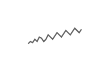
\begin{tikzpicture}[x=0.08em, y=0.08em, line width=0.4pt]
                \draw[FooterGray] (0,3) -- (1,4) -- (2,3.5) -- (3,5) -- (4,4) -- (5,6) -- (6,5.5) -- (7,4) -- (8,5) -- (9,7) -- (10,6) -- (11,5) -- (12,6.5) -- (13,8) -- (14,7) -- (15,6) -- (16,7.5) -- (17,9) -- (18,8) -- (19,7) -- (20,8.5) -- (21,10) -- (22,9) -- (23,8) -- (24,9.5);
            \end{tikzpicture}%
        }%
        \hskip0.5cm%
    }%
    \vskip6pt%
}

%=============================================================================
% PACHETE
%=============================================================================
\usepackage[utf8]{inputenc}
\usepackage[T1]{fontenc}
\usepackage{amsmath, amssymb, amsthm}
\usepackage{mathtools}
\usepackage{bm}
\usepackage{tikz}
\usetikzlibrary{arrows.meta, positioning, shapes, calc, decorations.pathreplacing, shadings}
\usepackage{booktabs}
\usepackage{multirow}
\usepackage{array}
\usepackage{graphicx}
\usepackage{hyperref}
\usepackage{colortbl}
\usepackage{listings}
\lstset{language=Python, basicstyle=\ttfamily\scriptsize, keywordstyle=\color{MainBlue}\bfseries,
  commentstyle=\color{Forest}, stringstyle=\color{Crimson}, breaklines=true,
  frame=none, backgroundcolor=\color{VeryLightGray}, xleftmargin=2mm}
\hypersetup{colorlinks=true, linkcolor=MainBlue, urlcolor=MainBlue}
\graphicspath{{../../logos/}{../../charts/}{../../photos/}}
\hfuzz=2pt
\vfuzz=2pt

%=============================================================================
% COMANDA QUANTLET
%=============================================================================
\newcommand{\quantlet}[2]{%
    \hfill\href{#2}{%
        \raisebox{-0.15em}{
\includegraphics[height=0.7em]{ql_logo.png}}%
        \textcolor{MainBlue}{\tiny\ #1}%
    }%
}

%=============================================================================
% PAGINĂ DE TITLU PERSONALIZATĂ
%=============================================================================
\defbeamertemplate*{title page}{hybrid}[1][]
{
    \vspace{0.2cm}
    \begin{center}
        \href{https://www.ase.ro}{
\includegraphics[height=1.0cm]{ase_logo.png}}\hspace{0.3cm}%
        \href{https://theida.net}{
\includegraphics[height=1.0cm]{ida_logo.png}}\hspace{0.3cm}%
        \href{https://blockchain-research-center.com}{
\includegraphics[height=1.0cm]{brc_logo.png}}\hspace{0.3cm}%
        \href{https://www.ai4efin.ase.ro}{
\includegraphics[height=1.0cm]{ai4efin_logo.png}}\hspace{0.3cm}%
        \href{https://ipe.ro/new}{
\includegraphics[height=1.0cm]{acad_logo.png}}\hspace{0.3cm}%
        \href{https://www.digital-finance-msca.com}{
\includegraphics[height=1.0cm]{msca_logo.png}}%
    \end{center}

    \vspace{0.6cm}

    \begin{center}
        \begin{minipage}{0.1\textwidth}
            \centering
            \href{https://quantlet.com}{
\includegraphics[height=1.1cm]{ql_logo.png}}
        \end{minipage}%
        \begin{minipage}{0.78\textwidth}
            \centering
            {\LARGE\bfseries\usebeamercolor[fg]{title}\inserttitle}

            \vspace{0.3cm}

            {\usebeamerfont{subtitle}\usebeamercolor[fg]{title}\insertsubtitle}
        \end{minipage}%
        \begin{minipage}{0.1\textwidth}
            \centering
            \href{https://quantinar.com}{
\includegraphics[height=1.1cm]{qr_logo.png}}
        \end{minipage}
    \end{center}

    \vspace{0.6cm}

    \hspace{0.5cm}{\usebeamerfont{author}\insertauthor}

    \vspace{0.3cm}

    \hspace{0.5cm}\begin{minipage}[t]{0.9\textwidth}
        \raggedright\small\insertinstitute
    \end{minipage}
}

%=============================================================================
% MEDII DE TEOREME
%=============================================================================
\theoremstyle{definition}
\setbeamertemplate{theorems}[numbered]
\newtheorem{defn}{Definiție}
\newtheorem{thm}{Teoremă}
\newtheorem{prop}{Propoziție}
\newtheorem{rmk}{Observație}

%=============================================================================
% MINIPAGE CENTRAT
%=============================================================================
\newenvironment{cminipage}[1]{%
    \par\noindent\hfill\begin{minipage}{#1}\ignorespaces
}{%
    \end{minipage}\hfill\null\par
}

%=============================================================================
% COMENZI PERSONALIZATE
%=============================================================================
\newcommand{\E}{\mathbb{E}}
\newcommand{\Var}{\text{Var}}
\newcommand{\Cov}{\text{Cov}}
\newcommand{\Corr}{\text{Corr}}
\newcommand{\R}{\mathbb{R}}
\newcommand{\N}{\mathbb{N}}
\newcommand{\Z}{\mathbb{Z}}
\newcommand{\B}{\mathbf{B}}
\newcommand{\imark}{\textcolor{MainBlue}{\textbullet}}

%=============================================================================
% INFORMAȚII TITLU
%=============================================================================
\title[Statistică pe Piețe Financiare]{Statistică pe Piețe Financiare}
\subtitle{Estimatori de Volatilitate}
\author[D.T. Pele, A. Amza]{\texorpdfstring{\begin{tabular}[t]{@{}l@{}}Daniel Traian PELE \\ Antoaneta Amza\end{tabular}}{Daniel Traian PELE, Antoaneta Amza}}
\institute{Academia de Studii Economice din București\\
IDA Institute Digital Assets\\
Blockchain Research Center\\
AI4EFin Artificial Intelligence for Energy Finance\\
Academia Română, Institutul de Prognoză Economică\\
MSCA Digital Finance}
\date{}

\begin{document}

% Pagina de titlu (fără antet/subsol)
{
\setbeamertemplate{headline}{}
\setbeamertemplate{footline}{}
\begin{frame}
    \titlepage
\end{frame}
}

%=============================================================================
% MOTIVAȚIE
%=============================================================================
\section{Motivație}

\begin{frame}{Volatilitatea}
\begin{columns}[T]
\begin{column}{0.55\textwidth}
\begin{itemize}
    \item Volatilitatea este o măsură statistică a \textbf{dispersiei randamentelor} pentru un activ financiar sau indice de piață dat.
    \item Reprezintă gradul de variație a prețului unui activ în timp.
    \item Estimatori dezvoltați pentru piețele financiare:
    \begin{itemize}
        \item Volatilitatea istorică, Parkinson, Garman-Klass
        \item Rogers-Satchell, Yang-Zhang
        \item Volatilitatea realizată, modele GARCH / HEAVY
        \item Volatilitate stocastică cu salturi, volatilitate implicită
    \end{itemize}
\end{itemize}
\end{column}
\begin{column}{0.42\textwidth}
\begin{center}
    {\small\textit{[Cutremurul și tsunamiul din 2011, T\={o}hoku, Japonia]}}
\end{center}
\end{column}
\end{columns}
\end{frame}

%=============================================================================
% CUPRINS
%=============================================================================
{
\setbeamertemplate{headline}{%
    \vskip10pt%
    \hbox to \paperwidth{%
        \hskip0.5cm%
        \hfill%
        \hskip0.5cm%
    }%
    \vskip4pt%
    {\color{FooterGray}\hrule height 0.4pt}%
}
\begin{frame}{}
    {\color{FooterGray}\hrule height 0.4pt}

    \vspace{0.3cm}

    {\Large\textcolor{IDAred}{\textbf{Cuprins}}}

    \vspace{0.4cm}

    \begin{itemize}
        \item Motivație \checkmark
        \item Estimatori de volatilitate
        \item Concluzii și teme
        \item Bibliografie
    \end{itemize}
\end{frame}
}

%=============================================================================
% ESTIMATORI DE VOLATILITATE
%=============================================================================
\section{Estimatori de volatilitate}

\begin{frame}{Volatilitatea istorică}
\begin{itemize}
    \item Măsoară \textbf{dispersia sau variabilitatea} randamentelor pe o perioadă specificată din trecut.
    \item Volatilitatea istorică se calculează ca \textbf{abaterea standard} a randamentelor anterioare:
    \[
    \sigma = \sqrt{\frac{1}{n-1}\sum_{t=1}^{n}(r_t - \bar{r})^2}
    \]
    \item \textbf{Anualizarea volatilității:} Deoarece volatilitatea este adesea exprimată pe bază anuală, volatilitatea zilnică poate fi anualizată folosind:
    \[
    \sigma_{\text{annual}} = \sigma_{\text{daily}} \times \sqrt{T}
    \]
    \begin{itemize}
        \item $T$ este numărul de perioade de tranzacționare dintr-un an (de obicei 252 de zile de tranzacționare).
        \item $\sigma_{\text{daily}}$ este abaterea standard a randamentelor zilnice.
    \end{itemize}
    \item \textbf{Limitările volatilității istorice:}
    \begin{itemize}
        \item Performanța trecută poate să nu prezică volatilitatea viitoare.
        \item Nu ia în considerare șocurile sau schimbările de regim ale pieței.
    \end{itemize}
\end{itemize}
\end{frame}

\begin{frame}{Volatilitatea istorică}
\begin{center}
    {\small\textit{[Două grafice: (1) Prețul de închidere AAPL și Volatilitatea pe 30 de zile (linie albastră preț, linie roșie volatilitate, 2022-01 până la 2023-09); (2) Randamentele logaritmice AAPL și Volatilitatea pe 30 de zile (randamente verzi, volatilitate roșie)]}}
\end{center}
\end{frame}

\begin{frame}{Regula rădăcinii pătrate a timpului}
\begin{columns}[T]
\begin{column}{0.65\textwidth}
\begin{itemize}
    \item Concept fundamental în managementul riscului financiar și în finanțele cantitative.
    \item Oferă o metodă de \textbf{scalare a volatilității} pe diferite orizonturi de timp, presupunând randamente IID care urmează o distribuție normală.
    \item Presupunem randamente $r_t \sim \mathcal{N}(\mu, \sigma^2)$ i.i.d.
    \item Randamentul total pe $n$ perioade: $R_n = r_1 + r_2 + \ldots + r_n$
    \item Deoarece randamentele sunt IID:
    $\E[R_n] = n\mu$, \  $\Var(R_n) = n\sigma^2$
    \item Abaterea standard pe $n$ perioade:
    $\sigma_n = \sqrt{\Var(R_n)} = \sqrt{n}\,\sigma$
    \item Volatilitatea se scalează cu \textbf{rădăcina pătrată a timpului}.
    \item În practică: $\sigma_{\text{annual}} = \sigma_{\text{daily}} \times \sqrt{N}$, unde $N$ este numărul de zile de tranzacționare (de obicei 252).
\end{itemize}
\end{column}
\begin{column}{0.32\textwidth}
\begin{center}
    {\small\textit{[Portretul lui Louis Bachelier]}}
\end{center}
\end{column}
\end{columns}
\end{frame}

\begin{frame}{Estimatorul Parkinson}
\begin{itemize}
    \item Estimatorii tradiționali se bazează adesea exclusiv pe prețurile de închidere, omițând potențial informații valoroase conținute în cadrul perioadei de tranzacționare.
    \item Parkinson (1980) a introdus un estimator care utilizează \textbf{prețurile maxime și minime} dintr-o perioadă.
    \item \textbf{Ipoteze:} tranzacționare continuă, drift zero în procesul de preț.
    \item Prin utilizarea intervalului---diferența dintre prețul maxim și cel minim---surprinde variabilitatea intra-perioadă a prețului mai eficient decât estimatorii bazați exclusiv pe prețuri de închidere.
    \[
    \sigma_P = \frac{1}{\sqrt{4\ln 2}}\sqrt{\frac{1}{n}\sum_{t=1}^{n}\left(\ln\left(\frac{H_t}{L_t}\right)\right)^2}
    \]
    \begin{itemize}
        \item $H_t$ este prețul maxim din ziua $t$.
        \item $L_t$ este prețul minim din ziua $t$.
        \item $n$ este numărul de perioade.
    \end{itemize}
\end{itemize}
\end{frame}

\begin{frame}{Aplicații}
\begin{itemize}
    \item \textbf{Estimarea volatilității pe piețele financiare:} utilizat pe scară largă atunci când prețurile de închidere nu surprind pe deplin mișcările de preț; oferă estimări mai precise (Fiszeder \& Perczak, 2013; Jacob \& Vipul, 2008).
    \item \textbf{Analiza comparativă a estimatorilor de volatilitate:} adesea inclus alături de estimatorii Garman-Klass și Rogers-Satchell (Lapinova \& Saichev, 2017; Vasileiou, 2023).
    \item \textbf{Managementul riscului și evaluarea instrumentelor derivate:} utilizat pentru evaluarea instrumentelor derivate (Jacob \& Vipul, 2008; Vasileiou, 2023).
    \item \textbf{Strategii de previziune și tranzacționare:} integrat în modele de previziune (Fiszeder \& Perczak, 2013; Jacob \& Vipul, 2008).
    \item \textbf{Aplicații pe piețele emergente:} deosebit de util acolo unde datele pot fi mai puțin fiabile (Jacob \& Vipul, 2008; Yang \& Zhang, 2000).
\end{itemize}
\end{frame}

\begin{frame}{Estimatorul Garman-Klass}
\begin{itemize}
    \item Încorporează \textbf{prețurile OHLC} (Open, High, Low, Close) pentru a oferi o estimare mai precisă a volatilității sub ipoteza de drift zero (Garman \& Klass, 1980):
    \[
    \sigma_{GK} = \sqrt{\frac{1}{n}\sum_{t=1}^{n}\left[0.5\left(\ln\left(\frac{H_t}{L_t}\right)\right)^2 - (2\ln 2 - 1)\left(\ln\left(\frac{C_t}{O_t}\right)\right)^2\right]}
    \]
    \item \textbf{Derivare:} Modelul Mișcării Browniene Geometrice (GBM) cu drift zero ($\mu=0$) și tranzacționare continuă.
    \item Ideea cheie: descompunerea varianței totale în componente care surprind diferite aspecte ale mișcărilor de preț.
    \item Sub GBM, modificările logaritmice ale prețului sunt distribuite normal.
    \item Varianța totală:
    \[
    \sigma^2 = \Var\!\left(\ln\frac{C_t}{O_t}\right) + \Var\!\left(\ln\frac{H_t}{L_t}\right) - 2\,\Cov\!\left(\ln\frac{C_t}{O_t},\, \ln\frac{H_t}{L_t}\right)
    \]
    \item Garman și Klass au derivat valorile așteptate ale acestor componente și le-au combinat pentru a minimiza varianța.
\end{itemize}
\end{frame}

\begin{frame}{Avantaje și limitări}
\begin{columns}[T]
\begin{column}{0.48\textwidth}
\begin{block}{Eficiență și avantaje}
\begin{itemize}
    \item Mai eficient decât estimatorii bazați doar pe prețuri de închidere sau pe intervale maxim-minim.
    \item Încorporează prețurile de deschidere și de închidere.
    \item Reduce varianța estimatorului.
    \item Aproximativ \textbf{de 7,4 ori mai eficient} decât estimatorul închidere-la-închidere și mai eficient decât Parkinson.
    \item Ia în considerare atât intervalul intra-zilnic, cât și mișcările deschidere-închidere.
\end{itemize}
\end{block}
\end{column}
\begin{column}{0.48\textwidth}
\begin{alertblock}{Ipoteze și limitări}
\begin{itemize}
    \item GK presupune \textbf{randament așteptat zero}.
    \item Tranzacționare continuă.
    \item Fără salturi de preț.
    \item Fără distorsiuni ale prețului de deschidere.
    \item Încălcările (gap-uri overnight, salturi) pot introduce distorsiuni.
\end{itemize}
\end{alertblock}
\end{column}
\end{columns}
\end{frame}

\begin{frame}{Estimatorul Rogers-Satchell}
\begin{itemize}
    \item Estimatorul Rogers-Satchell:
    \[
    \sigma_{RS} = \sqrt{\frac{1}{n}\sum_{t=1}^{n}\left[\ln\!\left(\frac{H_t}{C_t}\right)\ln\!\left(\frac{H_t}{O_t}\right) + \ln\!\left(\frac{L_t}{C_t}\right)\ln\!\left(\frac{L_t}{O_t}\right)\right]}
    \]
    \item \textbf{Aplicații:}
    \begin{itemize}
        \item Managementul riscului: evaluarea riscului de deținere/tranzacționare.
        \item Evaluarea opțiunilor: volatilitate precisă pentru evaluarea instrumentelor derivate.
        \item Optimizarea portofoliului: informarea alocării activelor.
    \end{itemize}
    \item \textbf{Avantaje:}
    \begin{itemize}
        \item Ajustarea pentru drift: ia în considerare drift-ul în procesul de preț.
        \item Încorporează mai multe puncte de preț (OHLC).
    \end{itemize}
    \item \textbf{Limitări:}
    \begin{itemize}
        \item Cerințe de date: necesită date OHLC detaliate.
    \end{itemize}
    \item \textbf{Ipoteze:} prețul activului urmează o Mișcare Browniană Geometrică cu drift.
\end{itemize}
\end{frame}

\begin{frame}{Aplicații}
\begin{itemize}
    \item \textbf{Estimarea volatilității pe piețele emergente:} utilizat frecvent (\"{O}zt\"{u}rk et al., 2016).
    \item \textbf{Analiză comparativă:} estimări robuste în cazul mișcărilor extreme de preț (Lapinova \& Saichev, 2017).
    \item \textbf{Aplicații pe piețele de criptomonede:} surprinde caracteristicile unice ale volatilității (Cadenas-Morales, 2022).
    \item \textbf{Managementul riscului și evaluarea instrumentelor derivate:} precis pe piețele de acțiuni și opțiuni (Fa{\l}dzi\'{n}ski \& Osi\'{n}ska, 2016).
    \item \textbf{Strategii de previziune și tranzacționare:} performanță îmbunătățită (Banerjee, 2023).
\end{itemize}
\end{frame}

\begin{frame}{Estimatorul Yang-Zhang}
\begin{itemize}
    \item Estimatorul Yang-Zhang (Yang \& Zhang, 2000) combină volatilitatea \textbf{overnight} (închidere-deschidere) cu o medie ponderată a volatilității Rogers-Satchell și a volatilității deschidere-închidere.
    \item \textbf{De 14 ori mai eficient} decât estimatorul închidere-la-închidere:
    \[
    \sigma_{YZ} = \sqrt{\sigma_O^2 + k\,\sigma_C^2 + (1-k)\,\sigma_{RS}^2}
    \]
    \item $\sigma_{YZ}$: volatilitatea estimată Yang-Zhang.
    \item \textbf{Varianța overnight:}\quad
    $\sigma_O^2 = \frac{1}{T-1}\sum_{t=1}^{T}\!\left(\ln\!\frac{O_t}{C_{t-1}} - \overline{\ln\!\frac{O_t}{C_{t-1}}}\right)^{\!2}$
    \item \textbf{Varianța deschidere-închidere:}\quad
    $\sigma_C^2 = \frac{1}{T-1}\sum_{t=1}^{T}\!\left(\ln\!\frac{C_t}{O_t} - \overline{\ln\!\frac{C_t}{O_t}}\right)^{\!2}$
    \item \textbf{Varianța Rogers-Satchell:}\quad
    $\sigma_{RS}^2 = \frac{1}{n}\sum_{t=1}^{n}\!\left[\ln\!\frac{H_t}{C_t}\ln\!\frac{H_t}{O_t} + \ln\!\frac{L_t}{C_t}\ln\!\frac{L_t}{O_t}\right]$
    \item $k = \frac{\alpha - 1}{\alpha + \frac{T+1}{T-1}}$: Factor de ponderare, de obicei $k = 0.34$.
\end{itemize}
\end{frame}

\begin{frame}{Estimatori de volatilitate: Exemplu}
\begin{center}
    {\small\textit{[Grafic cu estimatori de volatilitate rulantă pentru AAPL. Linii: Historical\_Vol (albastru), Parkinson\_Vol (portocaliu), Garman\_Klass\_Vol (verde), Rogers\_Satchell\_Vol (roșu), Yang\_Zhang\_Vol (violet). Interval de date 2019-01 până la 2022-07. Logo Q în colțul din dreapta jos.]}}
\end{center}
\end{frame}

%=============================================================================
% RENTABILITATE AJUSTATĂ LA RISC
%=============================================================================
\section{Rentabilitate ajustată la risc}

\begin{frame}{Indicatorul Sharpe}
\begin{itemize}
    \item Indicatorul Sharpe măsoară \textbf{randamentul excesiv} al unui activ față de rata fără risc, ajustat pentru risc (volatilitate).
    \item Este o măsură larg utilizată a \textbf{performanței ajustate la risc}.
    \[
    SR_t = \frac{\bar{R}_t - R_f}{\sigma_t}
    \]
    \begin{itemize}
        \item $\bar{R}_t$ este randamentul mediu al activului pe perioada $t$.
        \item $R_f$ este rata fără risc, de obicei bazată pe obligațiuni de stat.
        \item $\sigma_t$ este volatilitatea randamentelor pe perioada $t$.
    \end{itemize}
    \item Un \textbf{indicator Sharpe mai mare} indică o performanță ajustată la risc mai bună (Sharpe, 1966).
\end{itemize}
\end{frame}

\begin{frame}{Interpretarea indicatorului Sharpe}
\begin{itemize}
    \item Valori mai mari indică randamente ajustate la risc mai bune.
    \item Permite compararea investițiilor cu niveluri diferite de risc.
\end{itemize}

\vspace{0.3cm}

\begin{center}
\begin{tabular}{>{\centering\arraybackslash}p{3cm} >{\centering\arraybackslash}p{4cm}}
\toprule
\textbf{Indicatorul Sharpe} & \textbf{Interpretare} \\
\midrule
\rowcolor{Crimson!30} $SR < 0$ & Mai rău decât rata fără risc \\
\rowcolor{Orange!30} $0 - 0.5$ & Slab \\
\rowcolor{Amber!30} $0.5 - 1$ & Acceptabil \\
\rowcolor{Forest!20} $1 - 2$ & Bun \\
\rowcolor{Forest!40} $> 2$ & Excelent \\
\bottomrule
\end{tabular}
\end{center}
\end{frame}

\begin{frame}{Cadru matematic}
\begin{itemize}
    \item \textbf{Randamentul așteptat al unui portofoliu:}
    \[
    \E[R_p] = \sum_{i=1}^n w_i \cdot \E[R_i]
    \]
    \begin{itemize}
        \item $w_i$: Ponderea activului $i$.
        \item $\E[R_i]$: Randamentul așteptat al activului $i$.
        \item $n$: Numărul de active.
    \end{itemize}
    \item În practică, se folosesc adesea mediile randamentelor istorice:
    \[
    \E[R_i] \approx \frac{1}{T}\sum_{t=1}^T r_{i,t}
    \]
    \item Anualizat din randamente zilnice:
    \[
    \E[R_i]_{\text{annual}} = \E[R_i]_{\text{daily}} \times 252
    \]
\end{itemize}
\end{frame}

\begin{frame}{Volatilitatea portofoliului}
\begin{itemize}
    \item Volatilitatea portofoliului ține cont de \textbf{corelațiile dintre active}:
    \[
    \sigma_p = \sqrt{\sum_{i=1}^n\sum_{j=1}^n w_i\, w_j\, \sigma_i\, \sigma_j\, \rho_{ij}}
    \]
    \item În notație matriceală:
    \[
    \sigma_p = \sqrt{\mathbf{w}^T \Sigma\, \mathbf{w}}
    \]
    \begin{itemize}
        \item $\mathbf{w}$: Vectorul ponderilor activelor.
        \item $\Sigma$: Matricea de covarianță a randamentelor.
    \end{itemize}
    \item Anualizat din volatilitatea zilnică:
    \[
    \sigma_{\text{annual}} = \sigma_{\text{daily}} \times \sqrt{252}
    \]
\end{itemize}
\end{frame}

\begin{frame}{Optimizarea portofoliului}
\begin{itemize}
    \item \textbf{Frontiera eficientă} --- Portofolii care:
    \begin{itemize}
        \item Maximizează randamentul așteptat pentru un nivel dat de risc.
        \item Minimizează riscul pentru un nivel dat de randament așteptat.
        \item Fiecare punct de pe frontieră este o alocare unică de portofoliu.
        \item Portofoliile sub frontieră sunt suboptimale.
    \end{itemize}
\end{itemize}
\end{frame}

\begin{frame}{Frontiera eficientă}
\begin{itemize}
    \item Analizând aceste active:
    \begin{itemize}
        \item \textbf{SPY}: S\&P 500 (acțiuni americane de mare capitalizare)
        \item \textbf{QQQ}: Nasdaq 100 (tehnologie)
        \item \textbf{GLD}: Aur
        \item \textbf{TLT}: Obligațiuni de stat pe termen lung
        \item \textbf{VNQ}: Imobiliare
    \end{itemize}
\end{itemize}

\vspace{0.2cm}

\begin{center}
{\small
\begin{tabular}{lccc}
\toprule
\textbf{Activ} & \textbf{Randament (\%)} & \textbf{Volatilitate (\%)} & \textbf{Indicatorul Sharpe} \\
\midrule
SPY & 14.33 & 19.35 & 0.637 \\
QQQ & 19.57 & 24.04 & 0.7309 \\
GLD & 11.62 & 14.31 & 0.6725 \\
TLT & $-0.37$ & 16.16 & $-0.1469$ \\
VNQ & 8.23 & 22.75 & 0.2738 \\
\bottomrule
\end{tabular}
}
\end{center}

\vspace{0.1cm}

{\small Descărcarea datelor de preț de la 2018-01-01 la 2025-03-04. S-au descărcat 1801 zile de date. Generarea a 10000 de portofolii aleatorii.}
\end{frame}

\begin{frame}{Frontiera eficientă}
\begin{center}
    {\small\textit{[Grafic de tip scatter cu Frontiera Eficientă a Portofoliilor. Axa X: Volatilitate anualizată (Abatere standard), Axa Y: Randament așteptat anualizat. Codificat prin culoare după Indicatorul Sharpe (bară de culoare de la 0 la 0,8+). Stea roșie: Portofoliul Optim (Sharpe: 0,9070)]}}
\end{center}
\end{frame}

\begin{frame}{Portofoliul optim}
\begin{center}
    {\small\textit{[Grafic cu bare pentru Alocarea Activelor din Portofoliul Optim. SPY: 47,7\%, QQQ: 33,4\%, GLD: 17,4\%, TLT: 0,9\%, VNQ: 0,6\%. Randament: 14,62\%, Volatilitate: 13,91\%, Indicatorul Sharpe: 0,9070]}}
\end{center}
\end{frame}

%=============================================================================
% CONCLUZII ȘI TEME
%=============================================================================
\section{Concluzii și teme}

\begin{frame}{Concluzii}
\begin{itemize}
    \item \textbf{Randamentele} reprezintă metrica fundamentală pentru evaluarea performanței activelor.
    \item \textbf{Estimatorii de volatilitate} măsoară amplitudinea fluctuațiilor prețurilor activelor, ajutând la cuantificarea nivelului de risc de piață.
    \item Volatilitatea este esențială pentru înțelegerea \textbf{incertitudinii de piață} și constituie piatra de temelie a strategiilor de management al riscului.
    \item Estimarea precisă a volatilității susține o mai bună \textbf{evaluare a instrumentelor derivate}, gestionarea portofoliului și luarea deciziilor strategice pe piețe turbulente.
    \item Traderii și analiștii se bazează pe previziunile de volatilitate pentru a \textbf{stabili limite de risc} și a ajusta dinamic strategiile.
    \item Randamentele și estimatorii de volatilitate sunt date de intrare fundamentale pentru algoritmi din \textbf{tranzacționarea de înaltă frecvență} și sisteme automate, ghidând deciziile de cumpărare/vânzare și optimizând portofoliile.
\end{itemize}
\end{frame}

\begin{frame}{Teme}
\begin{center}
    {\small\textit{[Imaginea timbrului Petrache Poenaru]}}
\end{center}
\end{frame}

\begin{frame}{Calculul randamentelor --- Diavolul se ascunde în detalii}
\begin{itemize}
    \item Prețul unei acțiuni la momentul $t$ este $P_t = \$100$. Pe parcursul următoarelor trei perioade, randamentele compuse continuu sunt $r_{t+1} = 0.1$, $r_{t+2} = -0.05$ și $r_{t+3} = 0.02$.
    \item Calculați prețul acțiunii la momentele $t+1$, $t+2$, $t+3$. Arătați calculele.
    \item Acum, presupuneți că randamentele simple pe aceleași perioade sunt $R_{t+1} = 0.1$, $R_{t+2} = -0.05$ și $R_{t+3} = 0.02$. Calculați prețurile.
    \item Comparați rezultatele --- Sunt identice? De ce sau de ce nu?
    \item Explicați implicațiile practice pentru orizonturi de timp mai lungi.
\end{itemize}
\end{frame}

\begin{frame}{Calculul randamentelor --- Diavolul se ascunde în detalii}
\begin{itemize}
    \item Vi se dă o serie temporală de prețuri ale acțiunilor $P_0, P_1, \ldots, P_n$.
    \item Derivați o formulă generală pentru calculul randamentului total compus continuu de la momentul $0$ la momentul $n$.
    \item Cum se raportează aceasta la randamentele individuale pe perioade?
    \item Explicați cum se aplică conceptul de \textbf{aditivitate temporală} la randamentele compuse continuu.
    \item De ce este această proprietate dezirabilă în modelarea financiară?
\end{itemize}
\end{frame}

\begin{frame}{Volatilitate și risc --- Dincolo de elementele de bază}
\begin{itemize}
    \item Definiți volatilitatea în contextul piețelor financiare. Raportați la discuția despre risc.
    \item De ce este volatilitatea considerată o măsură a riscului? Ce tip de risc surprinde?
    \item Discutați diferite moduri de a estima volatilitatea.
    \item Avantaje și dezavantaje ale utilizării datelor istorice?
    \item Care sunt alte abordări (menționați cel puțin două)?
\end{itemize}
\end{frame}

\begin{frame}{Volatilitate și risc --- Dincolo de elementele de bază}
\begin{itemize}
    \item Două active A și B. Activul A are un randament așteptat mai mare și o volatilitate mai mare. Cum decideți în care să investiți? Explicați aversiunea la risc.
    \item Un portofoliu din X și Y cu ponderi $w_X$ și $w_Y$ ($w_X + w_Y = 1$). Volatilități $\sigma_X$ și $\sigma_Y$, corelație $\rho_{XY}$.
    \item Derivați formula pentru volatilitatea portofoliului $\sigma_P$.
    \item Explicați cum poate diversificarea să reducă volatilitatea portofoliului.
\end{itemize}
\end{frame}

\begin{frame}{Regula rădăcinii pătrate a timpului --- Când da și când nu}
\begin{itemize}
    \item Explicați regula rădăcinii pătrate a timpului pentru scalarea volatilității. Scrieți formula. Definiți toate variabilele.
    \item Care sunt ipotezele principale?
    \item O acțiune are o volatilitate zilnică de 1,2\%. Estimați volatilitățile săptămânală, lunară și anuală (5, 22, 252 de zile de tranzacționare). Arătați calculele.
    \item Acum imaginați-vă că randamentele sunt autocorelate pozitiv. Volatilitatea anuală reală ar fi mai mare sau mai mică decât estimarea?
    \item Cum afectează autocorelația scalarea volatilității?
\end{itemize}
\end{frame}

%=============================================================================
% BIBLIOGRAFIE
%=============================================================================
\section{Bibliografie}

\begin{frame}{Bibliografie}
{\scriptsize
\begin{thebibliography}{99}
\bibitem{jiang2013} Jiang, Z., Xu, Y., \& Zhang, Y. (2013). Volatility forecasts using range-based estimators. \textit{Journal of Futures Markets}, 33(3), 231--252.
\bibitem{molnar2012} Moln\'{a}r, P. (2012). Properties of range-based volatility estimators. \textit{International Review of Financial Analysis}, 25, 1--12.
\bibitem{sheraz2022} Sheraz, M. et al. (2022). Volatility dynamics of non-linear volatile time series and application to financial markets. \textit{Entropy}, 24(10), 1410.
\bibitem{miralles2018} Miralles-Quir\'{o}s, M.M. et al. (2018). Diversification and benefits of using exchange-traded funds. \textit{International Journal of Financial Engineering}, 23(2), 153--166.
\bibitem{faldzinski2016} Fa{\l}dzi\'{n}ski, M. \& Osi\'{n}ska, A. (2016). Volatility estimators in econometric analysis of risk on financial markets. \textit{Dynamic Econometric Models}, 16, 1--20.
\bibitem{changchien2011} Changchien, S.Y. et al. (2011). Improving Hull and White's method for estimating implied volatility. \textit{Journal of Futures Markets}, 30(6), 635--646.
\bibitem{vasileiou2023} Vasileiou, E. (2023). Are the intraday volatility estimations more representative of financial market risk? \textit{3rd Oxford Symposium}, Istanbul.
\end{thebibliography}
}
\end{frame}

\begin{frame}{Bibliografie (cont.)}
{\scriptsize
\begin{thebibliography}{99}
\bibitem{lapinova2017} Lapinova, I. \& Saichev, A. (2017). Comparative statistics of Garman-Klass, Parkinson, and Rogers-Satchell volatility estimators. \textit{Cogent Physics}, 4(1).
\bibitem{meilijson2008} Meilijson, I. (2008). The Garman-Klass volatility estimator revisited. \textit{arXiv preprint}.
\bibitem{banerjee2023} Banerjee, A. (2023). Does public sentiment impact stock price forecasting and trading strategies? \textit{Journal of Economics, Management and Finance}, 23(1), 108--134.
\bibitem{cadenas2022} Cadenas-Morales, E. (2022). Bitcoin volatility estimate applying Rogers-Satchell range model. \textit{International Journal of Financial Innovation and Risk Management}, 12(1), 49--79.
\bibitem{ozturk2016} \"{O}zt\"{u}rk, H. et al. (2016). Extreme value volatility estimators and their empirical performance. \textit{International Journal of Economics and Finance}, 8(8), 73.
\bibitem{yang2000} Yang, D. \& Zhang, Q. (2000). Drift-independent volatility estimation based on high, low, open, and close prices. \textit{Journal of Business}, 73(3), 477--492.
\end{thebibliography}
}
\end{frame}

\end{document}